\uuid{krLE}
\titre{Question d'optimisation}
\theme{fonctions de plusieurs variables}
\auteur{}
\datecreate{2024-04-18}
\organisation{AMSCC}
\contenu{
	
\texte{ 	Soit la fonction $f$ définie sur $\mathcal{D} \subset \R^2$ par 
	$$f(x,y) = y^2-x^2y+x^2$$
	où $\mathcal{D} = \{ (x,y) \in \R^2 \, , \, x^2-1 \leq y \leq 1-x^2\}$. }
	
	\begin{enumerate}
		\item \question{ Parmi les trois domaines représentés graphiquement ci-dessus, lequel est susceptible de représenter $\mathcal{D}$ ?
		
		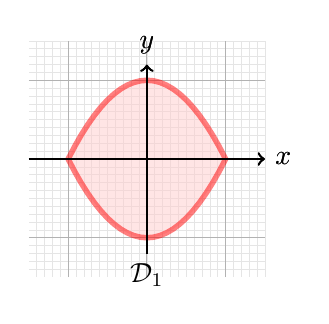
\begin{tikzpicture}[domain=-1:1]
			\draw[->,thick] (-1.5,0) -- (1.5,0) node[right] {$x$};
			\draw[->,thick] (0,-1.2) -- (0,1.2) node[above] {$y$};
			\draw[very thin, style=gray!20,  step=0.1] (-1.5,-1.5) grid(1.5,1.5);
			\draw[thin,gray!60]  (-1.5,-1.5) grid(1.5,1.5);
			\filldraw[fill=red!20, draw=red, line width = 2pt, opacity = 0.5] plot [domain=-1:1] (\x,{1-\x*\x})  -- plot [domain=1:-1] (\x,{\x*\x-1}) ;
			\draw[->,thick] (-1.5,0) -- (1.5,0) node[right] {$x$};
			\draw[->,thick] (0,-1.2) -- (0,1.2) node[above] {$y$};
			\draw (0,-1.2) node[below]{$\mathcal{D}_1$} ;
		\end{tikzpicture} \hfill
		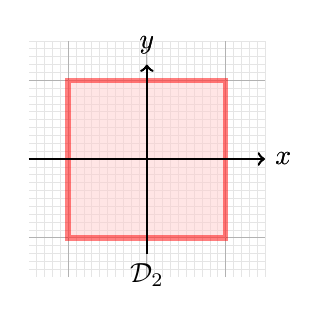
\begin{tikzpicture}[domain=-1:1]
			\draw[->,thick] (-1.5,0) -- (1.5,0) node[right] {$x$};
			\draw[->,thick] (0,-1.2) -- (0,1.2) node[above] {$y$};
			\draw[very thin, style=gray!20,  step=0.1] (-1.5,-1.5) grid(1.5,1.5);
			\draw[thin,gray!60]  (-1.5,-1.5) grid(1.5,1.5);
			\filldraw[fill=red!20, draw=red, line width = 2pt, opacity = 0.5] (1,1) -- (1,-1) -- (-1,-1) -- (-1,1) -- cycle ;
			\draw[->,thick] (-1.5,0) -- (1.5,0) node[right] {$x$};
			\draw[->,thick] (0,-1.2) -- (0,1.2) node[above] {$y$};
			\draw (0,-1.2) node[below]{$\mathcal{D}_2$} ;
		\end{tikzpicture} \hfill
		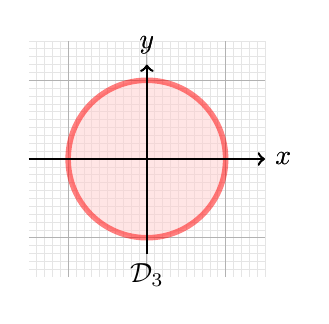
\begin{tikzpicture}[domain=-1:1]
			\draw[->,thick] (-1.5,0) -- (1.5,0) node[right] {$x$};
			\draw[->,thick] (0,-1.2) -- (0,1.2) node[above] {$y$};
			\draw[very thin, style=gray!20,  step=0.1] (-1.5,-1.5) grid(1.5,1.5);
			\draw[thin,gray!60]  (-1.5,-1.5) grid(1.5,1.5);
			\filldraw[fill=red!20, draw=red, line width = 2pt, opacity = 0.5] (0,0) circle (1) ;
			\draw[->,thick] (-1.5,0) -- (1.5,0) node[right] {$x$};
			\draw[->,thick] (0,-1.2) -- (0,1.2) node[above] {$y$};
			\draw (0,-1.2) node[below]{$\mathcal{D}_3$} ;
		\end{tikzpicture} }
		\reponse{
			Le domaine $\mathcal{D}$ est le domaine $\mathcal{D}_1$, dont le bord est constitué de deux branche de paraboles d'équation $y = x^2-1$ et $y = 1-x^2$.
		}
		\item  \question{ L'ensemble $\mathcal{D}$ est-il ouvert dans $\R^2$ ? fermé dans $\R^2$ ? Justifier très brièvement. }
		\reponse{
			Le domaine $\mathcal{D}$ est fermé dans $\R^2$ car le complémentaire de $\mathcal{D}$ est ouvert dans $\R^2$.
		}
		\item \question{ Justifier que $f$ admet un maximum global et un minimum global sur $\mathcal{D}$. }
		\reponse{
			La fonction $f$ est continue sur le domaine $\mathcal{D}$ qui est fermé et borné. Donc, $f$ admet un maximum global et un minimum global sur $\mathcal{D}$.
		}
		\item\question{  Vérifier que $(0,0)$ est l'unique point critique de $f$ dans l'intérieur du domaine  $\mathcal{D}$.  }
		\reponse{
			La fonction $f$ est de classe $\mathcal{C}^1$ sur $\mathcal{D}$ et on a $\dfrac{\partial f}{\partial x}(x,y) = -2xy+2x$ et $\dfrac{\partial f}{\partial y}(x,y) = 2y-x^2$. Pour déterminer les points critiques de $f$ dans l'intérieur de $\mathcal{D}$, on résout le système d'équations suivant :
			$$\left\{\begin{aligned}
			-2xy+2x & = 0 \\
			2y-x^2 & = 0
			\end{aligned}\right.$$
			Par substitution, on trouve : 
			$$\left\{\begin{aligned}
				-x^3+2x & = 0 \\
				2y &= x^2
			\end{aligned}\right.$$
			La première équation donne $x(x^2-2) = 0$ donc $x = 0$ ou $x = \pm \sqrt{2}$. Si $x = 0$, la deuxième équation donne $y = 0$. Si $x = \pm \sqrt{2}$, la deuxième équation donne $y = 2$. Or le point $(\sqrt{2},2)$ n'appartient pas à $\mathcal{D}$. Donc, l'unique point critique de $f$ dans l'intérieur de $\mathcal{D}$ est $(0,0)$.
		}
		\item \question{ La fonction $f$ admet-elle un extremum local sur l'intérieur de $\mathcal{D}$ ? }
		\reponse{
			On calcule les dérivées partielles secondes de $f$ :
			$$\dfrac{\partial^2 f}{\partial x^2}(x,y) = -2y+2 \quad \text{et} \quad \dfrac{\partial^2 f}{\partial y^2}(x,y) = 2$$
			et
			$$\dfrac{\partial^2 f}{\partial x \partial y}(x,y) = -2x.$$
			La matrice hessienne de $f$ évaluée en $(0,0)$ est
			$$H_f(0,0) = \begin{pmatrix}
			2 & 0 \\
			0 & 2
			\end{pmatrix}.$$
			donc son déterminant est $4 > 0$. Or $\dfrac{\partial^2 f}{\partial x^2}(0,0) = 2 > 0$. Donc d'après les conditions du second ordre, $(0,0)$ est un minimum local de $f$ sur l'intérieur de $\mathcal{D}$.
		}
		\item \texte{ Pour tout $x \in [-1;1]$, on pose $g(x) = f(x,1-x^2)$ et $h(x) = f(x,x^2-1)$.  }
		\begin{enumerate}
			\item \question{ Simplifier les expressions de $g(x)$ et $h(x)$. }
			\reponse{
				On a $g(x) = (1-x^2)^2-x^2(1-x^2)+x^2 = 2x^4-2x^2+1$ et $h(x) = (x^2-1)^2-x^2(x^2-1)+x^2 = 1$. 
			}
			\item \question{ \'Etudier les variations des fonctions $g$ et $h$ sur l'intervalle $[-1;1]$.  }
			\reponse{
				On a $g'(x) = 8x^3-4x$ et $h'(x) = 0$. Les points critiques de $g$ sont $-\frac{1}{\sqrt{2}}$, $0$ et $\frac{1}{\sqrt{2}}$. Donc $g$ est décroissante sur $[-1;-\frac{1}{\sqrt{2}}]$, croissante sur $[-\frac{1}{\sqrt{2}};0]$, décroissante sur $[0;\frac{1}{\sqrt{2}}]$ et croissante sur $[\frac{1}{\sqrt{2}};1]$. La fonction $h$ est constante égale à $1$ sur $[-1;1]$. On a $g\left( -\frac{1}{\sqrt{2}} \right) = g\left( \frac{1}{\sqrt{2}} \right) = \frac{1}{2}$ et $g(-1)=g(0)=g(1) = 1$. Donc $g$ admet un minimum global égal à $\frac{1}{2}$ sur $[-1;1]$ et un maximum global égal à $1$ sur $[-1;1]$. 
			}
			\item \question{ En déduire l'existence et le calcul d'un minimum et d'un maximum de la fonction $f$ sur le bord de $\mathcal{D}$.   }
			\reponse{
				La restriction de $f$ au bord de $\mathcal{D}$ est donnée par $g$ et $h$, selon qu'on se place sur la branche supérieure ou inférieure du bord de $\mathcal{D}$. Donc, $f$ admet un minimum global égal à $\frac{1}{2}$ et un maximum global égal à $1$ sur le bord de $\mathcal{D}$.
			}
		\end{enumerate}
		\item \question{ En déduire la valeur du minimum global de $f$ sur  $\mathcal{D}$ et la valeur du maximum global de $f$ sur   $\mathcal{D}$.  }
		\reponse{
			On a un minimum local de $f$ en $(0,0)$ égal à $0$, un minimum global de $f$ sur le bord de $\mathcal{D}$ égal à $\frac{1}{2}$ et un maximum global de $f$ sur le bord de $\mathcal{D}$ égal à $1$. Donc, le minimum global de $f$ sur $\mathcal{D}$ est $0$ et le maximum global de $f$ sur $\mathcal{D}$ est $1$.
		}
	\end{enumerate}
}